% siminos/spatiotemp/chapter/LC21blog.tex
% $Author: predrag $ $Date: 2021-12-24 01:25:20 -0500 (Fri, 24 Dec 2021) $

\section{Kittens' LC21blog}
\label{s:CL18blog}

Internal discussions of \refref{LC21} edits:
Move good text not used in \refref{LC21} to this file, for possible
reuse later.

\bigskip

Tentative title:    ``Is there anything cats cannot do?"

\begin{description}

\item[2016-11-18 Predrag]
A theory of turbulence that has done away with \emph{dynamics}?
We rest our case.

As a gentle introduction
for a reader too busy\rf{focusPOT} to study the book\rf{ChaosBook},
we
disguise a brief course on chaos theory as something everyone
understands, a Bernoulli coin toss, \refsect{s:coinToss}.

one determines the total number of
{\lattstate}s by computing the {\HillDet} \refeq{detBern0} of the
\emph{\jacobianOrb}

The observation that a Bernoulli system can be viewed as a discretization
of a first-order in time ODE, eq.~\refeq{1stepVecEq}, with solutions
whose temporal global linear stability is described by the {\jacobianOrb}
$\jMorb_{\zeit\zeit'}=\delta{F[\Xx]}_{\zeit}/\delta\ssp_{\zeit'}$, has
profound implications for dissipative \spt\ systems such as Navier-Stokes
and Kuramoto-Sivashinsky\rf{GuBuCv17}.

As we shall here have to traverse territory unfamiliar to many, we
follow Mephistopheles pedagogical dictum ``You have to say it three
times"\rf{GoetheIstuZim1806}, and sing our song thrice.

The deep insight here is that the two formulations of mechanics, the
for\-ward-in-time Hamiltonian evolution, and the global, Lagrangian,
{\templatt} formulation are related by the {\em Hill's formula}.

The deep insight
here is the realization that the {\em\HillDet}, \ie, the volume of the
{\em\jacobianOrb} (\reffig{fig:BernCyc2Jacob} and \ref{fig:catCycJacob})
partitions system's \statesp.

Next, we address two questions:
(i) how is the high-dimensional orbit \jacobianOrb\ $\jMorb$ related
to the temporal [$d\!\times\!d$] \jacobianM\ $\jMat$?
(\refsect{s:LC21Hill}),
and
(ii) how does one evaluate the orbit \jacobianM\ $\jMorb$?
(\refsects{sect:LC21recip1d}{sect:LC21recip1d}).

The theory is compactly summarized by its {\tzeta} \refeq{Isola90-13}
that counts Bravais lattices.

Still, when we think of a temporal lattice as `time': no dynamicist does
that. Embarrassing.

The dynamics is breathtakingly simple on the reciprocal lattice.
Spatial period-$\cl{}$
Bravais cell maps onto a regular $\cl{}$-gon in the reciprocal lattice. Time reversal fixes
the symmetric solutions to sit on the symmetry
axes, the boundaries of the fundamental domain.
Lattice shift $\shift_j$ maps out the $\Group$-orbit by running on
circles, and orbits visit the $1/2\cl{}$ wedge only once, so the points
in the fundamental domain represent an orbit each.

with all reciprocal
lattice Brillioun zone solutions {\orbit}s in an $1/n$ sliver of a
$\cl{}$-gon.

No self-respecting crystallographer would be drawing longer and longer
Bravais {\lattstate}s \refeq{reflSymOdd}-\refeq{reflSymEvens1} - they
eventually run off the sheet of paper, no matter how wide.
A professional crystallographer plots all {\lattstate}s snugly together
in the first Brillouin zone, where the translational orbit of a
{\lattstate} is -literally- a circle, symmetric  {\lattstate}s sit on
boundaries of point group's fundamental domain, and everything is
maximally diagonalized in term's of space group \Group\ irreps.

Consider
\[
\rho_{\vec{G}}(\vec{x})= e^{i\vec{G}\cdot\vec{r}(\vec{x})}
\,,
\]
where $\vec{G}$ is a reciprocal lattice vector. By definition,
$\vec{G}\cdot\vec{a}$ is an integer multiple of $2\pi$, $\rho_{\vec{G}}=1$ for
lattice vectors.
For any other state, reciprocal {\lattstate} is given by
\[
e^{i\vec{G}\cdot\vec{u}(\vec{x})} \neq 1
\,.
\]

When a
cube is a building block that tiles a $3D$ cubic lattice, it is referred
to as the `elementary' or `Wigner-Seitz' cell, and its Fourier transform
is called `the first Brillouin zone' in `the reciprocal space'.



%\item[2018-04-18 Predrag]
the time-reversal pairs
to be the complex-conjugate pairs in Fourier space, as \Cn{\infty} shift
moves them in opposite directions.

The eigenvectors of the translation operator which satisfy the
periodicity of the Bravais lattice % \refeq{2DBravLatt}
are plane waves of form:
\beq
f_\mathbf{k}(\mathbf{z}) = e^{i \mathbf{k} \cdot \mathbf{z}}
  \,, \quad
\mathbf{k} \in \overline{\lattice}
\,,
\ee{LC21:Rcpr1dEgnVect}
where the wave vector $\mathbf{k}$ is on the reciprocal lattice
$\overline{\lattice}$.

 A general plane wave does not
satisfy the periodicity, unless
\beq
e^{i {k} \cdot {R}} = 1
\, .
\ee{LC21:PrdicPlaneWave}
Since ${R}$ is a vector from the Bravais lattice $\lattice$, the wave
vector $\mathbf{k}$ must lie in the reciprocal lattice of $\lattice$:
\beq
\mathbf{k} \in \lattice^*
\,,\quad
\lattice^* =
\left\{ m \mathbf{b}\,|\,m \in \mathbb{Z}\right\} \, ,
\ee{LC21:RcprocalLattice}
where the primitive reciprocal lattice vectors $\mathbf{b}$ satisfies:
 \beq
\mathbf{b} \cdot \mathbf{a} = 2 \pi
\, .
\ee{LC21:RcprocalLattBasis}


% \item[2020-01-23 Predrag]
Barvinok \arXiv{/math/0504444}:
\\
Let $V$ be a $d$-dimensional real vector space with the scalar product
$\langle \cdot, \cdot \rangle$
and the corresponding Euclidean norm $\| \cdot\|$. Let $\lattice \subset V$ be a lattice
and let  $\lattice^{\ast} \subset V$ be the {\it dual} or the {\it reciprocal} lattice
\[
\lattice^{\ast}=\Bigl\{x \in V: \quad \langle x, y \rangle \in {\Bbb Z}
\quad
\mbox{ for all } \quad y \in \lattice \Bigr\}
\,.
\]

\item[2021-08-10 Han]
% \subsection
{\bf Reciprocal {\lattstate}}

An infinite {\lattstate} is periodic if the state is invariant under the action of a translation group.
A translation group can be described by a Bravais lattice, the vector in
which determines the direction and distance of the translation. When the dynamical system
has time translation symmetry, the defining equation of the system is invariant under translations.
So it is natural to use the eigenvectors of the translation operator to study the {\lattstate}s of the
system.

The eigenvectors of translation operators are plane waves defined on the lattice. But to study
the {\lattstate}s, we need to require that the plane wave also satisfies the periodic
condition. Generally, a $d$\dmn\ Bravais lattice can be described by:
\bea
{\lattice} = \left\{\sum_{i=1}^d n_i \mathbf{b}_i | n_i \in \mathbb{Z}\right\}
\,,
\eea
where $\mathbf{b}_i$ is the $i$th primitive vector of the Bravais lattice.
And a plane wave on the $d$\dmn\ lattice is:
\bea
f_\mathbf{k}(\mathbf{z}) = e^{i \mathbf{k} \cdot \mathbf{z}}
\, ,
\eea
where $\mathbf{z}$ is the position of a lattice site, and $\mathbf{k}$ is the wave vector.
The periodicity given by the Bravais lattice $\lattice$ requires that:
\bea
f_\mathbf{k}(\mathbf{z}+\mathbf{R})
=f_\mathbf{k}(\mathbf{z})\,,
\quad
\mathbf{R} \in \lattice \,.
\eea
This condition can only be satisfied if the wave vector $\mathbf{k}$ exists on the
reciprocal lattice of the lattice $\lattice$:
\bea
\overline{\lattice} = \left\{ \sum_{j=i}^d n_i \mathbf{b}_i | n_i \in \mathbb{Z}\right\}
\,,
\eea
the basis vectors of which satisfy:
\bea
\mathbf{b}_i \cdot \mathbf{a}_j = 2 \pi \delta_{ij} \,.
\eea
Using these eigenvectors we can transform {\lattstate}s into reciprocal {\lattstate}s
by discrete Fourier transform.
Any {\lattstate} with the periodicity given by the Bravais lattice
$\lattice$ can be spanned by the plane waves with wave vectors in the
reciprocal lattice $\overline{\lattice}$. And since a {\lattstate} only has
values on lattice sites, we only need a finite number of plane waves to
span the {\lattstate}.
%For each {\lattstate} with periodicity given by a Bravais lattice,
%there exists a reciprocal {\lattstate}.

When we write period-$\cl{}$ {\lattstate}s as $\cl{}$\dmn\ vectors, and write the
shift operator $\shift$ as a $[\cl{} \times \cl{}]$ matrix \refeq{hopMatrix} which applies
cyclic permutation to the
{\lattstate}, the matrix representation of shift operators forms a permutation representation
of the cyclic translation group $\Cn{n}$. This permutation representation is a reducible
representation, i.e., it can be block diagonalized by a similarity transformation. Each block
on the diagonal is an irreducible representation (irrep).

The abelian group $\Cn{\cl{}}$ only has 1\dmn\ irreps. The permutation
representation of $\Cn{\cl{}}$ can be diagonalized by discrete Fourier transform. After the
transform the representation of the shift operator becomes,
\bea
\shift^{m}=
\left(
\begin{array}{ccccc}
1 \\
& \omega^m \\
& & \omega^{2m} \\
& & & \ddots \\
& & & & \omega^{(\cl{}-1)m}
\end{array}
\right) \,,
\quad
\omega=\e^{2\pi\mathrm{i}/\cl{}}
\,,
\eea
with {\lattstate}s projected onto 1\dmn\ subspaces
in which action of the shift operators is given by corresponding irrep.
As we transform the permutation representation of the shift operator into the block
diagonal form,
the {\lattstate}s
$(\ssp_{0},\ssp_{1},\ssp_{2},\dots,\ssp_{\cl{}-1})$
are spanned by the  Fourier modes basis,
with components
$(\cssp_{0},\cssp_{1},\cssp_{2},\dots,\cssp_{\cl{}-1})$.
When the shift operator acts on the {\lattstate}: $\Xx \to \shift \Xx$, the irreducible
representations act on the components in the corresponding subspace:
$\cssp_{k} \to \omega^k \cssp_{k}$.

%\subsubsection
{\bf Dihedral group}
%\label{sect:LC21irrepsDn}

In the $\cl{}$\dmn\ space of the period-$\cl{}$ {\lattstate}s, the permutation representation
of the Dihedral group \Dn{\cl{}} can be generated by the shift operator matrix representation
\refeq{hopMatrix} and the reflection operator matrix representation:
\bea
\Refl=
\left(
\begin{array}{ccccc}
 1 &&&&0\\
  &  &  & 0 & 1 \\
  &  & \reflectbox{$\ddots$} & 1 &  \\
  & 0 & \reflectbox{$\ddots$} &  &  \\
  0& 1 &  &  &  \\
\end{array}
\right) \,.
\eea

The Dihedral group $\Dn{\cl{}}$ has: 2 1\dmn\ irreps and $[(\cl{}-1)/2]$
2\dmn\ irreps if $\cl{}$ is odd,
or 4 1\dmn\ irreps and $(\cl{}/2-1)$ 2\dmn\ irreps if $\cl{}$ is even.
If $\cl{}$ is odd, the permutation representation can be block diagonalized into irreps:
$A_0 \oplus E_1 \oplus \dots \oplus E_{(\cl{}-1)/2}$.
If $\cl{}$ is even, the permutation representation can be block diagonalized into irreps:
$A_0 \oplus B_1 \oplus E_1 \oplus \dots \oplus E_{\cl{}/2-1}$.

        \PCpost{2021-09-02} {
Why do you mark 1/8 in
\reffigs{fig:BernC3}{fig:HLBernoulliC3InvariantOrbits}, when the
units are 1/7's? I see. You have $1/\sqrt{3}$ and $\pi$'s floating
around, unless you redefine units...
    }


\PCpost{2021-07-07}{
Experimenting with \refeq{Ryu17eq:1.3C} by:\\
%
%Kim \etal\rf{KiLePa03} prove that every finite index subgroup of
%the {infinite dihedral group} $\Dn{\infty}$
%\refeq{D_infty}
%\[
%\langle r, \Refl \mid \Refl r \Refl=r^{-1} \,,\; \Refl^2=1\rangle
%\]
%is
a flip across the $k$th axis, $k=0, 1, 2, \cdots, \cl{}-1$,
\bea
\mbox{dihedral } \Dn{\cl{}}:\quad
H_{\cl{},k}  &=&
\langle \shift, \Refl_k=\shift^k \Refl \mid \Refl_k \shift \Refl_k=\shift^{-1}
    \,,\;
           \shift^\cl{}=\Refl_k^2=1 \rangle
%            \continue
%            &&
%\cl{}=1, 2, 3, \cdots
\,,
\label{Ryu17eq:1.3C}
\eea
that Han had replaced with \refeq{KiLePa03H}
and $\cl{}$ with $|\cl{}|$ in \refeq{KiLePa03Index}.

%with index
%\beq
%|\Dn{\infty}/\Cn{\cl{}}| =  2\cl{}
%    \qquad \text{or} \qquad
%|\Dn{\infty}/\Dn{\cl{}}| = \cl{}
%\,.
%\ee{Ryu17eq:3.0}
}

\PCpost{2021-07-07}{
A presentation of the \emph{infinite dihedral group}\rf{KiLePa03} is
\beq
\Dn{\infty} = \left\langle {\shift_i,\Refl_j} \mid
      \shift_i\Refl_j= \Refl_j\shift_{-i};\;
      \Refl_j^2 = 1;\; i,j\in\integers
              \right\rangle
\,.
\ee{presntD_infty}
}

\item[2021-08-10 Predrag]
dropped:

Applying the projection operator
\(
\PP_{{0}-} = \frac{1}{2} (\unit-\Refl_{0})/2
\)
we obtain
a {\lattstate}
\beq
\cdots
\underline{{y}_{4}}\,\underline{{y}_{3}}\,\underline{{y}_{2}}\,\underline{{y}_{1}}\,
 \sitebox{0}
      {y}_{1} {y}_{2} {y}_{3} {y}_{4}  \cdots
\,,
\ee{latticeInf0-}
antisymmetric under reflection, where the
field
\(
\sitebox{0} =(\ssp_0-\ssp_0)/2 =0
\)
at the reflection lattice site $0$ vanishes by antisymmetry, while the rest,
\(
{y}_{j} =(\ssp_{j}-\ssp_{-j})/2
\,,
\)
are pairwise antisymmetric under the reflection $\Refl$. The underline
indicates the negative of, \ie, $\underline{{y}_{j}}=-{y}_{j}$.

Applying the antisymmetric projection operator
\(
\PP_{{1}-} = \frac{1}{2} (\unit-\Refl\shift)/2
\)
we obtain a {\lattstate}
\beq
\cdots
\underline{{y}_{4}}\,\underline{{y}_{3}}\,\underline{{y}_{2}}\,\underline{{y}_{1}}\,
        |
      {y}_{1} {y}_{2} {y}_{3} {y}_{4}  \cdots
\,,
\ee{latticeInf1-}
antisymmetric under reflection, where
\(
{y}_{j} =(\ssp_{j}-\ssp_{1-j})/2
\,,
\)
are pairwise antisymmetric under the reflection $\Refl_{1}$.

    \PCpost{2021-08-21}{
The old definition of Bernoulli $\Ssym{\zeit}$ in \refeq{LC21:1dPhi4}
conflicted with the definition \refeq{circ-m}. I changed \refeq{circ-m}
to current form.
    }

    \PCpost{2021-10-29}{Dropped:
Cat maps are beloved by ergodicists and statistical mechanicians because,
even though the field $(\coord_{\zeit},p_{\zeit})$ is 2\dmn, for integer
values of the stretching parameter $s$, a cat map has a finite alphabet
linear code, just like the Bernoulli map, and its
unit torus can be tiled by two rectangles,
    \PC{2020-12-17}{
Link to the ChaosBook.
    }
in analogy with the forward-in-time Bernoulli map subinterval
partitioning of \reffig{fig:BernPart}. From this it follows that all
admissible symbol {\brick}s can be generated as shifts of finite
type, and all periodic points determined and counted.

As all that is well known, and a side issue for this paper, we relegate
the details of the Hamiltonian cat map dynamics and \po\ counting to
??.
    \PC{2020-12-17}{
Link to the ChaosBook.
    }
Here we focus on reformulating the cat dynamics as
a temporal lattice (or discrete Lagrangian) problem, as we have done for
the Bernoulli system in \refsect{s:1D1dLatt}.
    }

    \PCpost{2021-10-12}{
    Please read our draft\rf{LC21}, and either follow
    our definition \refeq{1dLattStat} of {\em {\lattstate}},
    or replace it with some other definition.
    }

    \PCpost{2021-10-29}{Dropped:
The Lagrangian formulation requires only temporal {\lattstate}s
and their actions, replacing the phase space `cat map' \refeq{catMap}
by a `{\templatt}' lattice \refeq{OneCat}. The {\templatt} has no
generating partition analogue of the \AW\ partition for a Hamiltonian cat
map (see
    \PC{2020-12-17}{
Link to the ChaosBook.
    }
).
As we have shown here, no funky Hamiltonian \statesp\ partitioning magic
(such as
    \PC{2020-12-17}{
Link to the ChaosBook.
    }
) is needed to count the
{\lattstate}s of a \templatt. Not only are no such partitions needed to
solve the system, but the Lagrangian,
    }

    \PCpost{2021-08-12}{
    Sidney will chuckle at this comment:
    The usual $a\ssp_{\zeit}^2$ form \refeq{Hen-1dLattA} might be
    preferable, as the `$a$' is a stretching parameter, just like in
    \refeq{LC21:1dTemplatt}. See \refsect{sect:HamHenonMap}~{{\Henlatt}}.
%    The same for $\phi^4$ coupling constant in \refeq{LC21:1dPhi4}.
    }

    \PCpost{2021-08-17} {See \refeq{PCreflSymOdd}.
We also MUST explain the relation to literature, as in the post including
\refeq{PC:Ryu17eq:2.11}.
    }

    \PCpost{2020-12-17}{
Link to the ChaosBook? or drop?\\
In \refsect{s:catPV} we review the traditional cat map in its Hamiltonian
formulation.
(but relegate to the explicit \AW\ generating partition of the cat map
\statesp).

We evaluate and cross-check  {\HillDet}s by two methods, either the
`fundamental fact' evaluation, or by the
discrete Fourier transform diagonalization, \refsect{sect:LC21recip1d}.
    }

    \PCpost{2021-10-13}{
Is there a - sign specific to Sidney's definition of the
\Henon\ {\jacobianOrb}
Han and Predrag have to redefine both
\templatt\ and \henlatt\ {\jacobianOrb} throughout, so we do not pick up an
extraneous `-' sign for odd period {\lattstate}s.
%
See also \refeq{Pozrikidis14(1.1.3)}, and Pozrikidis\rf{Pozrikidis14}
\CBlibrary{Pozrikidis14} eq.~(1.8.2). The main thing is to have a Laplacian
with positive eigenvalues, right? Maybe not, the main thing is to
have hyperbolic eigenvalues for $s>2$. Rethink.
determinants in \po\ formulas.

%       Predrag                          3 feb 2005
$Z[\source]$ notation extracted from \emph{lattFTnotat.tex},
called \emph{by lattFT.tex}.
% \Chapter{lattFT}{3feb2005}{Lattice field theory}

, in field theorist's parlance, $\Ssym{z}$ are `sources', and

The {\jacobianOrb} $\jMorb[\Xx]$ is best understood by starting with the
period-$\cl{}$ Bravais cell stability.

As in \refsect{sect:fundFact}, the {\fundPip} given the stretching of the
\cl{}\dmn\ \statesp\ unit hyper-cube $\Xx\in[0,1)^\cl{}$ by the
{\jacobianOrb} counts {\lattstate}s, with the {\admissible} {\lattstate}s
of period $\period{}$ constrained to field values within
$0\leq\ssp_\zeit<1$. The {\fundPip} contains images of all {\lattstate}s
$\Xx_\Mm$, which are then translated by integer winding numbers $\Mm$
into the origin, in order to satisfy the fixed point condition
\refeq{tempFixPoint}.

    }

    \PCpost{2021-10-21}{
Han, RECHECK all $\Ssym{\zeit}$, as well as formulas starting with
\refeq{1stepNonlimTemp}!!! Bernoulli $\Ssym{\zeit}$ in
\refeq{LC21:1dPhi4} conflicted with the old definition \refeq{circ-m}, so
I changed \refeq{circ-m}.

When the force is proportional to displacement, that is, when Hooke's law
is obeyed, the spring is said to be linear, the potential is quadratic.

A matrix $\jMat$ with no eigenvalue on the unit circle is called
hyperbolic.

Ignoring (mod~1) for a moment, we can use
\refeq{LC21PerViv2.1b} to eliminate
$p_{\zeit}$ from \refeq{LC21PerViv2.1a}
and rewrite the kicked rotor equation as the

For the problem at
hand, it pays to go from the Hamiltonian (configuration, momentum) phase
space formulation to the discrete Lagrangian
$(\ssp_{\zeit-1},\ssp_{\zeit})$ formulation.

\emph{temporal lattice} condition

`Temporal' again refers to the discretized time 1$d$ lattice

In atomic physics applications, the values of the angle $\coord$
differing by integers are identified, but the momentum $p$ is unbounded.
In dynamical systems theory one compactifies the momentum as well, by
adding $(\mbox{mod}\;1)$ to \refeq{LC21PerViv2.1a}, as for the Bernoulli map
\refeq{n-tuplingMap}. This reduces the phase space to a square
$[0,1)\times [0,1)$ of unit area, with the opposite edges identified,
\ie, 2-torus.

Thom-Anosov diffeomorphism

Cat maps with the same $s$ are equivalent
up to a similarity transformation, so it suffices to work out a single
convenient realization, as we shall do here for the
\PV\rf{PerViv} `two-configuration representation'
\refeq{LC21PerViv}.

    }

    \PCpost{2021-11-29} {
    Might need to introduce the inverse temperature $\beta = 1/T$ and the
    free energy $F$, as in \refeq{NKHM15ZJ}, multiplied by `volume' $N$
    the number of lattice sites;
\[
  Z[\source]	= e^{W[\source]}
  \,,\qquad
  W[\source] = \beta N F[\Xx]
\]
    So, $W[\source]$ is not the `free energy'.

Hill's formula here is the discrete Hill's formula\rf{MacMei83,BolTre10}
\refeq{MacMei83(17)}.

The temporal Bernoulli {\jacobianOrb} %\refeq{1stepVecEq},
$\jMorb=\partial/\partial\zeit-(s-1)\,\shift^{-1}$ is a differential
operator whose determinant one usually computes by a Fourier transform
diagonalization (see \refsect{sect:LC21recip1d}). The Fourier discretization
approach goes all the way back to Hill's 1886 paper\rf{Hill86};
    }

\PCpost{2021-11-29} {
                    {\color{red}
!!!WARNING!!!
Following Han \refeq{HLcorrectOrbJac}, we are changing the sign of the
action $\action[\Xx]$ and the {\jacobianOrb}, as in \refeq{LC21:1dTempFT},
THROUGHOUT! (Totally Predrag's fault).
This makes \catlatt\ and {$\phi^4$} theory action strictly positive
for
${s}>2$, as
needed for the probability interpretation \refeq{ProbConf}.
                    }
Han, Sidney and Predrag have to redefine
\templatt, \catlatt\ and \henlatt\ {\jacobianOrbs} throughout, to avoid the
extraneous `-' sign for odd period {\lattstate}s.
%
See also \refeq{Pozrikidis14(1.1.3)}, and Pozrikidis\rf{Pozrikidis14}
\CBlibrary{Pozrikidis14} eq.~(1.8.2).
    }

\PCpost{2016-11-08} {
Say: THE BIG DEAL is

for $d$\dmn\ field theory, symbolic dynamics is not one temporal sequence
with a huge alphabet, but $d$\dmn\ {\spt} tiling by a finite alphabet
   }

\PCpost{2021-12-27} {removed:\\
%\subsection
{\bf {\HillDet}: time-evolution evaluation}
%not used: \label{s:LC21HillHam}

However, in classical and statistical mechanics, one often computes the
{\HillDet} using a  Hamiltonian, or `transfer matrix' formulation.

Define
\[  %\beq
\hat{\xx}_\zeit
=
\left[\begin{array}{l}
 {\ssp}_{\zeit-1}\\
 {\ssp}_\zeit
 \end{array}\right]
,\quad
\hat{\mathsf{\Ssym{}}}_\zeit
=
    \left[\begin{array}{l}
    {0}\\
 {\Ssym{}}_{\zeit}
 \end{array}\right]
\,,
\] %\ee{PV2catlattJ1}
where the hat $\hat{~}$~ indicates a $2$\dmn\
`two-configuration'\rf{PerViv} lattice site $\zeit$ state.

The $1$\dmn\ field theory 3-term recurrence \refeq{LC21:1dTempFT} written
in the \PV\rf{PerViv} `two-configuration representation'
\refeq{LC21PerViv}.


$\mathbf{\jMorb}_1$ is the spatial
$[\speriod{}\!\times\!\speriod{}]$ {\jacobianOrb} of
$d=1$ \templatt\ form \refeq{tempCatFix},


This proves that $\det\hat{\mathbf{\jMorb}}$ of the
`Hamiltonian' or `two-configuration'
$[2\speriod{}\cl{}\times2\speriod{}\cl{}]$ `phase space'
\jacobianOrb\ $\hat{\mathbf{\jMorb}}$ defined by \refeq{eq:orbitJPVJxS}
equals the `Lagrangian' {\HillDet} of the
$[\speriod{}\cl{}\times\speriod{}\cl{}]$ \jacobianOrb\
$\mathbf{\jMorb}$.

While the setting is classical,
such deterministic field-theory advances offer new semi-classical
approaches to quantum field theory and many-body problems.

    }

    \HLpost {2021-12-26} {
I think \refeqs{LC21PerViv2.1b}{LC21PerViv2.1a} should be written as:
\bea
\coord_{\zeit+1} &=& \coord_{\zeit} + p_{\zeit+1} \qquad  (\mbox{mod}\;1), \\
p_{\zeit+1} &=& p_{\zeit} + P(\coord_{\zeit}) \,.
\eea
Otherwise the angle of the rotor $\coord$ is not constrained to $[0,1)$.
\\Predrag: you are right, corrected.
}

\bigskip\bigskip
\item[2021-12-29 Predrag]

The \statesp\ \pS\ of a $\Dn{\infty}$ invariant dynamical is union of
4 subspaces of {\lattstate}s 4 distinct symmetries
(see \reffig{fig:symmLattStates})
\beq
\pS = \pS_{a} \cup \pS_{o} \cup \pS_{ee} \cup \pS_{ee}
\,,
\ee{pSunion}
where

\noindent
$\qquad \Xx\in\pS_{a}\quad\;$
    {\em no reflection symmetry} \refeq{reflSymNo},
                                 see \reffig{fig:1dLatStatC_5}
\\ \qquad\qquad\qquad
orbit $p=\{\Xx, \shift\Xx, \cdots, \shift_{\cl{}-1}\Xx,
       \Refl\Xx, \Refl_1\Xx, \cdots, \Refl_{\cl{}-1}\Xx\}$

\noindent
$\qquad \Xx\in\pS_{o}\quad\;$
    {\em odd period, reflection-symmetric:} \refeq{reflSymOdd}
                                            see \reffig{fig:symmLattStates}
\\ \qquad\qquad\qquad
orbit $p=\{\Xx, \shift\Xx, \cdots, \shift_{\cl{}-1}\Xx\}$

\noindent
$\qquad \Xx\in\pS_{ee}\quad$
    {\em even period, even reflection-symmetric:} \refeq{reflSymEvens0}
\\

\noindent
$\qquad \Xx\in\pS_{eo}\quad$
    {\em even period, odd reflection-symmetric:} \refeq{reflSymEvens1}.

Let $\pS_{a}$ be the set of pairs of asymmetric orbits
 \refeq{reflSymNo}, each element of
the set a forward-in-time orbit and the time-reversed orbit.
If prime cycle $p \in \pS_{a}$ exists, it and each of its repeats counts
as 1:
\beq
1/\zeta_{p}(t) =
\exp \Big(-\sum_{r=1}^{\infty} \, \frac{1}{2\cl{p}r}t^{2\cl{p}r}\Big)
    =
\sqrt{1-t^{2\cl{p}}}
\,.
\ee{zeta_p(a)}

prime {\lattstate} $p \in \pS_{o}$ exists,
{\lattstate} invariant under the dihedral group $H_{\cl{},k}$, $\cl{p}$
values of $k$
\beq
1/\zeta_{p}(t) =
\exp \Big(-\sum_{r=1}^{\infty} \,
                     \frac{1}{r}t^{\cl{p}r}
      \Big) =
\exp \Big(-\sum_{r=1}^{\infty} \,
                     \frac{t^{\cl{p}}}{1-t^{\cl{p}}}
      \Big)
\,.
\ee{zeta_p(o)}

prime cycle $p \in \pS_{ee}$ exists
\beq
1/\zeta_{p}(t) =
\exp \Big(-\sum_{m=1}^{\infty} \left\{
       N_{2m-1, 0}\,t^{2m-1}
       + \left(N_{2m,0}+N_{2m,1}\right)\,\frac{ t^{2m}}{2}
                               \right\}\Big)
\,.
\ee{zeta_p(ee)}


Let $\pS_{s}$ be the collection of finite orbits with time
reversal (flip) symmetry, and $\pS_{a}$ be the collection of the pairs of
orbits without time reversal symmetry, each an orbit and the flipped
orbit. A finite \orbit\ $p$ is a periodic points set
\[
p = \{\ssp, \map(\ssp), \dots, \map^{\cl{p}-1}(\ssp)\}
\]
if $p \in \pS_{s}$, and
\[
p = \{\ssp, \map(\ssp), \dots, \map^{k-1}(\ssp)\} \cup
\{\Refl(\ssp), \map\circ\Refl(\ssp), \dots, \map^{k-1}\circ\Refl(\ssp)\}
\]
if $p \in \pS_{a}$, where $k=\cl{p}/2$.

If $p \in \pS_{s}$,
\beq
\zeta_{p}(t) =
\sqrt{\frac{1}{1-t^{2\cl{p}}}}\exp\left(\frac{t^{\cl{p}}}{1-t^{\cl{p}}}\right)
\,,
\ee{ZetaO1}

The product form of the zeta function is:
\beq
1/\zeta_{\mbox{\footnotesize KLP}}(t) =
\prod_{p_1\in {O_1}}\sqrt{1-t^{2\cl{p_1}}}
      \;\exp\left(-\frac{t^{\cl{p_1}}}{1-t^{\cl{p_1}}}\right)
\prod_{p_2\in \pS_{a}} (1-t^{\cl{p_2}})
\,.
\ee{ZetaProd}
========================================================================


\bigskip\bigskip
========================================================================
%    \item[2021-08-26 Han]
How to count the number of {\lattstate}s for \templatt?

\emph{No symmetry} {\lattstate}s \HillDet:
\[
N_\cl{} = \prod_{j=0}^{\cl{}-1} \left( s - 2\cos\frac{2\pi j}{\cl{}}\right)
\,.
\]
The products of eigenvalues for the $\Cn{\cl{}}$ discrete Fourier
case follows from \refeq{TableOfISP13952-2}:
\beq
\prod_{j=0}^{\cl{}-1} \left( s - 2\cos\frac{2\pi j}{\cl{}}\right)
= (\ExpaEig^{\cl{}/2}-\ExpaEig^{-\cl{}/2})^2
\,,
\ee{eigsProduct}
It's a square, because of the  $\Dn{\cl{}}$ symmetry.
Consider even, odd casses, use $\cos0=1$, $\cos\pi=-1$,
$\cos(-\theta)=\cos\theta$. The product over non-trivial eigenvalues is:
\bea
\cl{}=2m
     &&
M_{\cl{},0} =
 \prod_{j=1}^{m-1}\left({s}-2\cos\frac{\pi{j}}{m}\right)
      =  \frac{|\ExpaEig^{\cl{}/2}-\ExpaEig^{-\cl{}/2}|}
              {{\mu}\sqrt{{\mu}^2+4}}
\,,
\label{LC21:eigsProdEven}
\eea

\bea
\cl{}= 2m-1
     &&
M_{\cl{},1} =
 \prod_{j=1}^{m-1}\left({s}-2\cos\frac{2j\pi}{2m-1}\right)
     = \frac{|\ExpaEig^{\cl{}/2}-\ExpaEig^{-\cl{}/2}|}
              {{\mu}}
\,,
\label{LC21:eigsProdOdd}
\eea

Next, look at the \emph{symmetric} {\lattstate}s {\HillDet}s:

For odd $\cl{}=2m-1$,
\bea
N_{\cl{},1} = \prod_{j=0}^{m-1} \left(s-2\cos\frac{2\pi j}{\cl{}}\right)
={\mu}M_{\cl{},1}
\,.
\eea
For $\cl{}=2m$,
\bea
N_{\cl{},1} &=& \prod_{j=0}^{m-1} \left(s-2\cos\frac{2\pi j}{\cl{}}\right)
            \continue
N_{\cl{},0} &=& % \prod_{j=0}^{m} \left(s-2\cos\frac{2\pi j}{\cl{}}\right) =
                (s+2)\,N_{\cl{},1}
\,,
\eea
and
\bea
\frac{1}{2}\left(N_{\cl{},0}+
N_{\cl{},1} \right)
= \frac{\mu^2+5}{2}\prod_{j=0}^{m-1} \left(s-2\cos\frac{2\pi j}{\cl{}}\right)
= \frac{\mu^2+5}{2\mu}
\sqrt{\frac{\left(\ExpaEig^{\cl{}} + \ExpaEig^{-\cl{}} - 2\right)}
           {\mu^2+4}}
\,.
\eea
The number of {\lattstate}s can be written as polynomials:
For $\cl{}=2m-1$:
\bea
N_{\cl{},0} &=&
\mu\left(\ExpaEig^{\cl{}/2}-\ExpaEig^{-\cl{}/2}\right)
\continue
&=&
\mu^2\ExpaEig^{-1/2}\left(\ExpaEig^{m}-\ExpaEig^{-m+1}\right)
\,.
\eea
For $\cl{}=2m$:
\bea
\frac{1}{2}\left(N_{\cl{},0}+
N_{\cl{},1} \right)&=&
\frac{s+3}{2(\ExpaEig-\ExpaEig^{-1})}
\left(\ExpaEig^{\cl{}/2}-\ExpaEig^{-\cl{}/2}\right)
\continue
&=&
\frac{{\mu}^2+5}{2{\mu}\sqrt{{\mu}^2+4}}
\left|\ExpaEig^{m}-\ExpaEig^{-m}\right|
\,.
\eea
Now we can compute the $h(t)$ from \refeq{KLPzetaExp}
\bea
h(t) &=& \sum_{m=1}^{\infty} \left[
       N_{2m-1, 0}\,t^{2m-1}
       + \left(N_{2m,0}+N_{2m,1}\right)\,\frac{ t^{2m}}{2}
                               \right]
\continue
&=&
\mu\frac{\ExpaEig^{1/2} t}{1-\ExpaEig t^2}
-\mu\frac{\ExpaEig^{-1/2}t}{1-\ExpaEig^{-1}t^2}
\continue
&&+
\frac{\mu^2+5}{2(\ExpaEig-\ExpaEig^{-1})}\frac{\ExpaEig t^2}{1- \ExpaEig t^2}
-\frac{\mu^2+5}{2(\ExpaEig-\ExpaEig^{-1})}\frac{\ExpaEig^{-1} t^2}{1- \ExpaEig^{-1} t^2}
\,.
\eea
Using \refeq{KLPzetaFact} we have the symmetric {\lattstate}s
part of the Kim-Lee-Park zeta function. Expanding
this zeta function using \refeq{HLFlipGeneratingFunction}, we have:
\bea
- t \frac{\partial}{\partial t}(\ln e^{-h(t)}) &=&
t + 6 t^2 + 12 t^3 + 36 t^4 + 55 t^5 +144 t^6
\continue
&&+ 203 t^7 + 504 t^8 + 684 t^9
+1650 t^{10} + \dots
\,,
\eea
which is in agreement with \refeq{HLFlipGeneratingFunction}
and \reftab{tab:Bmack93Fixed}.

%%%%%%%%%%%%%%%%%%%%%%%%%%%%%%%%%%%%%%%%%%%%%%%%%%%%%%
\subsection{Counting {\lattstate}s}
\label{sect:LC21poCounts}    % derived from blogCats.tex {sect:PeriodicPsCount}


Given the {\tzeta} \refeq{KLPzeta} we can count the
number of {\lattstate}s from the generating function:
    \PC{2021-08-25}{
    We have the counts of the Bravais {\lattstate}s $N_\cl{}$,
    $N_{\cl{},k}$ already, from \refeq{N_nkCount}, so why don't we
    reverse the logic, start here, and get the zeta function
    \refeq{KLPzetaFact} by integration? Mention that this is an
    example of Lind zeta function\rf{Lind96} \refeq{LindZeta}
    without ever writing it down, so we do not have to explain it? It's a
    side issue for us, really.
    }
\beq
\frac{-t\frac{d}{dt}(1/\zeta_{\Refl}(t))}{1/\zeta_{\Refl}(t)}
= \sum_{\cl{}=1}^\infty N_\cl{}t^{2\cl{}}
+ \sum_{\cl{}=1}^\infty\sum_{k=0}^{\cl{}-1}N_{\cl{},k}t^{\cl{}}
= \sum_{m=1}^\infty a_m t^m \, ,
\ee{LC21zetatopGenerating}
where the coefficients are:
% https://tex.stackexchange.com/questions/401201/difference-between-align-and-alignedt
\beq
a_m =
\left\{
\begin{array}{ll}
\sum_{k=0}^{m-1} N_{m,k}^{\Refl}
= m N_{m,0}^{\Refl}
\,,\quad & \mbox{$m$ is odd}
 \, ,\\
N_{m/2} + \sum_{k=0}^{m-1} N_{m,k}^{\Refl}
= N_{m/2} + \frac{m}{2} \left(N_{m,0}^{\Refl} + N_{m,1}^{\Refl}\right)
\,,\quad & \mbox{$m$ is even}
\,.
 \end{array}\right.
\ee{LC21zetatopCoefficients}
Using the product formula of {\tzeta} \refeq{ZetaProd} and
the numbers of orbits with length up to 5 from the \reftab{tab:Bmack93Fixed},
we can write the {\tzeta}:
\bea
1/\zeta_{\Refl}(t) &=&
\sqrt{1-t^2} \exp\left(-\frac{t}{1-t}\right) (1-t^4) \exp\left(-\frac{2t^2}{1-t^2}\right)
\left(\sqrt{1-t^6}\right)^3 \continue
&& \exp\left(-\frac{3t^3}{1-t^3}\right)(1-t^6)(1-t^8)^3
\exp\left(-\frac{6t^4}{1-t^4}\right) \continue
&& (1-t^8)^2(1-t^{10})^5\exp\left(-\frac{10t^5}{1-t^5}\right)
(1-t^{10})^6 \dots \, .
\eea
The generating function is:
\bea
\frac{-t\frac{d}{dt}(1/\zeta_{\Refl})}{1/\zeta_{\Refl}}
=
t + 7t^2 + 12t^3 + 41t^4 + 55t^5 + \dots \, ,
\eea
which is in agreement with \refeq{LC21zetatopCoefficients}, where the $N_\cl{}$ and $N_{\cl{}}^{\Refl}$
are the $C_\cl{}$ and $SF_\cl{}$ in the \reftab{tab:Bmack93Fixed}.

We are not able to retrieve the numbers of fixed points by their symmetry groups using this {\tzeta} \refeq{KLPzeta}, unless we rewrite the {\tzeta} with two variables:
\beq
\zeta_{\Refl}(t,u) =
\exp \Big(\sum_{\cl{}=1}^{\infty} \, \frac{N_{\cl{}}}{2\cl{}}t^{2\cl{}}
          +\sum_{\cl{}=1}^{\infty} \, \sum_{k=0}^{\cl{}-1}\,
                     \frac{N_{\cl{},k}}{\cl{}}u^{\cl{}} \Big)
\,.
\ee{LC21FlipZetaTU}
Using this {\tzeta} $\zeta_{\Refl}(t,u)$ we can write two generating functions:
\beq
\frac{-t\frac{\partial}{\partial t}(1/\zeta_{\Refl}(t,u))}{1/\zeta_{\Refl}(t,u)}
= \sum_{\cl{}=1}^\infty N_\cl{}t^{2\cl{}}
\, ,
\ee{LC21zetatopGeneratingT}
and
\beq
\frac{-u\frac{\partial}{\partial u}(1/\zeta_{\Refl}(t,u))}{1/\zeta_{\Refl}(t,u)}
= \sum_{\cl{}=1}^\infty\sum_{k=0}^{\cl{}-1}N_{\cl{},k}u^{\cl{}}
\, .
\ee{LC21zetatopGeneratingU}
Using the product formula of this {\tzeta} and the numbers of orbits with length
up to 5 from the \reftab{tab:Bmack93Fixed}, the Kim-Lee-Park zeta function is:
\bea
1/\zeta_{\Refl}(t,u) &=&
\sqrt{1-t^2} \exp\left(-\frac{u}{1-u}\right) (1-t^4) \exp\left(-\frac{2u^2}{1-u^2}\right)
\left(\sqrt{1-t^6}\right)^3 \continue
&& \exp\left(-\frac{3u^3}{1-u^3}\right)(1-t^6)(1-t^8)^3
\exp\left(-\frac{6u^4}{1-u^4}\right) \continue
&& (1-t^8)^2(1-t^{10})^5\exp\left(-\frac{10u^5}{1-u^5}\right)
(1-t^{10})^6 \dots \, .
\eea
And the generating function from this {\tzeta} is:
\bea
\frac{-u\frac{\partial}{\partial u}(1/\zeta_{\Refl}(t,u))}{1/\zeta_{\Refl}(t,u)}
=
u + 6u^2 + 12u^3 + 36u^4 + 55u^5 + \dots \, ,
\label{HLFlipGeneratingFunction}
\eea
which is in agreement with \refeq{LC21zetatopGeneratingU}, where the $N_{\cl{}}^{\Refl}$ is the $SF_{\cl{}}$
in the \reftab{tab:Bmack93Fixed}.

    \PCpost{2021-12-10} {
Form $(V'(\ssp_{\zeit})-\Ssym{\zeit})$ looks like the most convenient
definition of the ``$\Ssym{}$-centered" subregion $\pS_\Ssym{}$ potential,
applicable to both linear and nonlinear field theories?
    }

    \PCpost{2021-08-23} {
We have omitted ``Quotienting the temporal Bernoulli system''
    \refeq{1stepDiffEqBlog} from this paper.
    }

    \PCpost {2021-12-10} {
\beq
-\Box\,x_{\zeit}+a\,x_{\zeit}^2 - 2\,x_{\zeit} - \Ssym{\zeit} \,=\, 0
\,.
\ee{HenonLap2}

\beq
V(\Xx,\Mm) = \sum_{\zeit\in\lattice}\left(
\frac{g}{k}\ssp_{\zeit}^k - \ssp_{\zeit}^2 -\Ssym{\zeit}\,\ssp_\zeit\right)
    \,,\qquad
        \Ssym{\zeit} = -1
\,.
\ee{LC21BWcubic1}
Works also for \templatt:
\beq
V(\Xx,\Mm) = \sum_{\zeit\in\lattice}\left(
\frac{s}{2}\ssp_{\zeit}^2 - \ssp_{\zeit}^2 -\Ssym{\zeit}\,\ssp_\zeit\right)
 = \sum_{\zeit\in\lattice}\left(
\frac{s-2}{2}\ssp_{\zeit}^2 -\Ssym{\zeit}\,\ssp_\zeit\right)\,,
\ee{LC21BWcubic1}
    }

\subsection{{\HillDet}: fundamental parallelepiped evaluation}
\label{s:LC21fundFacteval}
% 2020-02-16 Predrag computed  using siminos/mathematica/Tensors.nb
As a concrete example
consider the Bravais lattice % \refeq{1DBravLatt}
with basis
vector

The {\em \jacobianOrb} is the $\delta/\delta\ssp_k$ derivative of the
{\henlatt} 3-term recurrence relation \refeq{jMorb1dFT}
\bea
\jMorb_p &=& - \shift + 2\,{\mathbb{X}}_p - \shift^{-1}
\,,
\label{Henlatt-orbitJac}
\eea
where ${\mathbb{X}}_p$ is a diagonal matrix with $p$-{\lattstate} $\ssp_k$ in the
$k$th row/column, and the `$1$'s in the upper right and lower left corners
enforce the periodic boundary conditions.

The action of the \henlatt\ {\jacobianOrb} can be hard to visualize,
as a period-2 {\lattstate} is a 2-torus,
period-3 {\lattstate} a 3-torus, \etc. Still, the {\fundPip} for the period-2
and period-3 {\lattstate}s, should suffice to
convey the idea. The {\fundPip} basis vectors \refeq{lattJac} are the
columns of $\jMorb$. The $[2\!\times\!2]$ {\jacobianOrb}
and its {\HillDet} follow from \refeq{Henlatt-2-cycle}
\beq
\jMorb =
 \left(\begin{array}{cc}
2\,\ssp_0   & -2 \\
         -2 & 2\,\ssp_1
 \end{array} \right)
\,,\quad
\Det\jMorb = 4\,(\ssp_0\ssp_1-1)
           = -4\,(a-3)
\,.
\ee{Henlatt-catFundPar2}
% $( 1+ \sqrt{a-3} )( 1- \sqrt{a-3} )-1 = -a+3$
The resulting {\fundPip} shown in \reffig{fig:Henlatt-catCycJacob}\,(a).
Period-3
{\lattstate}s for $s=3$ are contained in the half-open {\fundPip} of
\reffig{fig:Henlatt-catCycJacob}\,(b),
defined by the columns of $[3\!\times\!3]$
{\jacobianOrb}
\beq
\jMorb =
\left(
\begin{array}{ccc}
2\,\ssp_0 &-1           &-1 \\
         -1 & 2\,\ssp_1 &-1 \\
         -1 &-1           & 2\,\ssp_2
\end{array}
\right)
\,,
\qquad
\Det \jMorb
    = 8\,\ssp_0\ssp_1\ssp_2-2\,(\ssp_0+\ssp_2+\ssp_3)+2
\,,
\label{Henlatt-catFundPar3}
\eeq

\HLpost{2021-12-31}{
Note that in the {temporal lattice} reformulation, the Bernoulli system
involves two distinct lattices:
\begin{itemize}
  \item[(i)]
Any lattice field theory:
in the discretization \refeq{LattField}
 of the time continuum, one replaces \emph{any}
dynamical system's time-dependent field $\ssp(\zeit)\in\reals$ at time
$\zeit\in\reals$ by a discrete set of its values
$\ssp_\zeit=\ssp(a\,\zeit)$ at time instants $\zeit\in\integers$.
Here the index $\zeit$ is a \emph{coordinate} over which the field
$\ssp$ is defined.
  \item[(ii)]
Specific to the Bernoulli system: the site $\zeit$ field value
$\ssp_{\zeit}$ \refeq{n-tuplingMap} is confined to the unit interval
$[0,1)$, imparting integer lattice structure onto the intermediate
calculational steps in the extended \statesp\ \refeq{BerStretch} on which
the {\jacobianOrb} \jMorb\ \refeq{tempBern} acts.
\end{itemize}

    \PC{2021-10-25}{
    Combine the above with the \templatt\ \refpage{} discussion into a
    remark that temporal Bernoulli and \templatt\ aslo have a
    \emph{dynamical} \Dn{1} symmetry, not utilized in this paper, as
    nonlinear field theories such as \henlatt\ do not have such
    symmetries. Here we study only the symmetries of the floor, not the
    dancer.
    }
}

\subsection{{\HillDet}: Reciprocal lattice evaluation}

$\omega = e^{2i\pi/\cl{}}$

$\cssp_k=x_k+i\,y_k = |\cssp_k| e^{i\theta_k}$

$q_k=2\pi{k}/\cl{}$,

$\cl{}$ is the Bravais cell period

\bigskip

The temporal Bernoulli {\jacobianOrb} %\refeq{1stepVecEq},
$\jMorb=\partial/\partial\zeit-(s-1)\,\shift^{-1}$ is a differential
operator whose determinant one usually computes by a Fourier transform
diagonalization (see \refsect{sect:LC21recip1d}). The Fourier discretization
approach goes all the way back to Hill's 1886 paper\rf{Hill86}.

The first advantage of using the reciprocal lattice is that it provides a
way to compute the {\HillDet}.
If the \jacobianOrb\ \refeq{jacobianOrb} commutes with the translation
operator, the plane waves are eigenvectors of the \jacobianOrb. Using
these eigenvectors one can find the eigenvalues and the determinant of
the \jacobianOrb. In the $\cl{}$\dmn\ space of {\lattstate}s with
period-$\cl{}$, the one-lattice spacing translation operator is a shift
matrix \refeq{hopMatrix},
%\bea
%\shift
%=  \left(\begin{array}{ccccc}
%             0    &  1    &        &   &  \cr
%                  &  0    &   1    &   &  \cr
%                  &       &        & \ddots &  \cr
%                  &       &        & 0 & 1 \cr
%             1    &       &        &   & 0
%          \end{array} \right)
%\,,
%\eea
whose eigenvectors are plane waves $\tilde{e}_k$:
\bea
\shift\,\tilde{e}_k = \omega^{k} \tilde{e}_k \, .
\eea
For example, the eigenvalues of the {temporal Bernoulli}
{\jacobianOrb} \refeq{tempBern} are
% $(\id-{s}\,\shift^{-1})$ is given by:
% \jMorb =
\bea
({s}\id - {\shift})\,\tilde{e}_k
= ({s} - \omega^{k})\,\tilde{e}_k
\,,
\eea
and the {\HillDet} is simply a polynomial whose roots are the \cl{}th
roots of unity,
\bea
\Det({s}\id - {\shift})
=
\prod_{k=0}^{\cl{}-1} ({s} - \omega^{k})
=
s^{\cl{}} - 1
\,.
\eea
see \refeq{shift2n}.
The eigenvalues of the \templatt\
{\jacobianOrb} \refeq{tempCatFix} are:
\bea
(-\shift+{s}\,\id-\shift^{-1})\,\tilde{e}_k
=
({s} - 2\cos(2\pi k/\cl{}))\,\tilde{e}_k \, ,
\eea
and the {\HillDet} is:
\bea
\mbox{\templatt: }\quad
\Det(-\shift+{s}\,\id-\shift^{-1})
    &=&
\prod_{k=0}^{\cl{}-1} [{s} - 2\cos(2\pi k/\cl{})]
    \continue
    &=&
2 T_{\cl{}} \left({s}/{2}\right) - 2 \, ,
\eea
where $T_{\cl{}}$ is the Chebyshev polynomial of the first
kind.

%%%%%%%%%%%%%%%%%%%%%%%%%%%%%%%%%%%%%%%%%%%%%%%
%2021-12-31 Han: figSrc/han/Mathematica/LC21Figure/TemporalCatEigenvalueBand.nb
\begin{figure}\begin{center}
            \begin{minipage}[c]{0.3\textwidth}\begin{center}
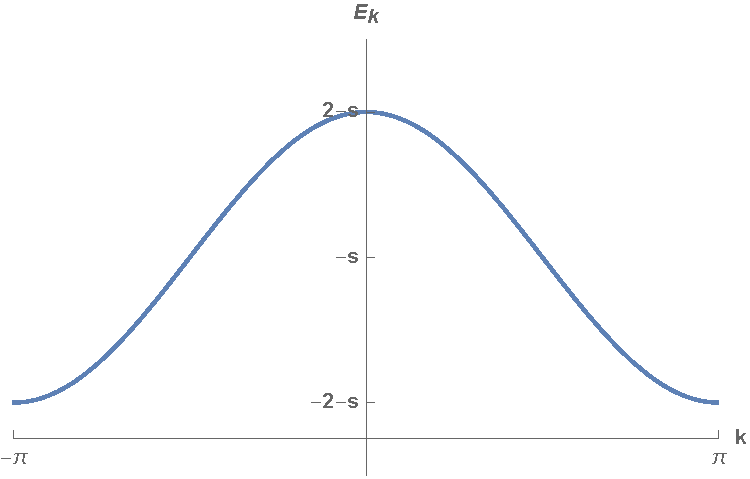
\includegraphics[width=1.0\textwidth]{HLTemplattBand}\\(a)
            \end{center}\end{minipage}
            \begin{minipage}[c]{0.3\textwidth}\begin{center}
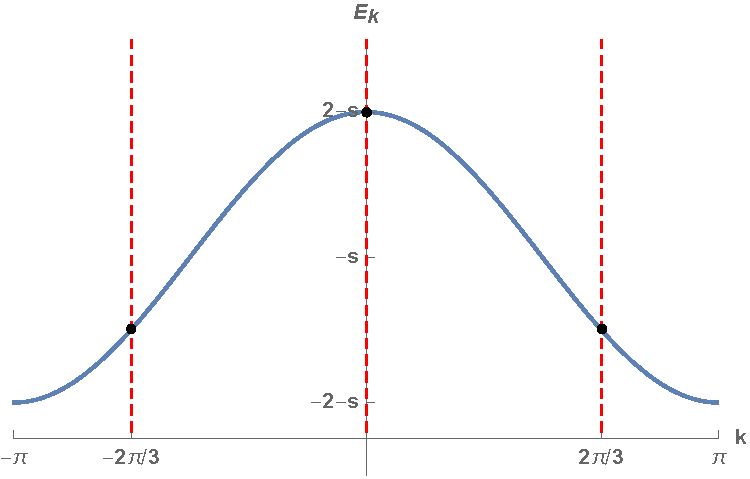
\includegraphics[width=1.0\textwidth]{HLTemplattBand3cycle}\\(b)
            \end{center}\end{minipage}
            \begin{minipage}[c]{0.3\textwidth}\begin{center}
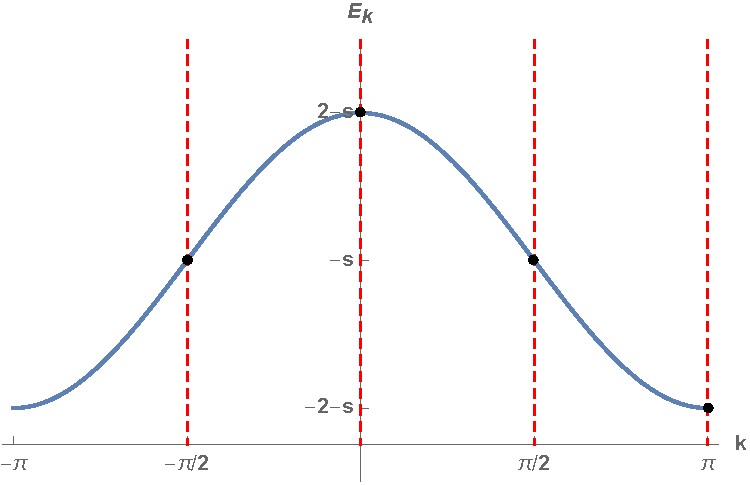
\includegraphics[width=1.0\textwidth]{HLTemplattBand4cycle}\\(c)
            \end{center}\end{minipage}
\end{center}
  \caption{\label{fig:LC21emplattBand}
(a) The eigenvalue $E_k$ of the \jacobianOrb\ on the infinite lattice as a function of the wave
vector $k$ in the first Brillouin zone. The \jacobianOrb\ has the reflection symmetry so the
eigenvalue is also invariant under the reflection $k\to -k$.
(b) For period 3 {\lattstate}s, the wave vectors of the eigenstates exist on the reciprocal lattice
spanned by $2\pi/3$. These lattice sites are labeled by the red dashed lines. There are only
3 period 3 eigenstates, with eigenvalues $s+1$, $s-2$ and $s+1$.
(c) For period 4 {\lattstate}s, the wave vectors of the eigenstates exist on the reciprocal lattice
spanned by $\pi/2$. These lattice sites are labeled by the red dashed lines. There are only
4 period 4 eigenstates, with eigenvalues $s$, $s-2$, $s$ and $s+2$.
$k=\pi$ and $k=-\pi$ are different by a reciprocal lattice translation, so they are a same
wave vector and should be only counted once.
          }
\end{figure}
%%%%%%%%%%%%%%%%%%%%%%%%%%%%%%%%%%%%%%%%%%%%%%%

Explain \reffig{fig:LC21emplattBand}.

        \PC{2021-09-02} {
I think I prefer some version of the identity \refeq{TableOfISP13952},
\refeq{HillDetOrbJ},
no mention of Chebyshev polynomials. Not important, will revisit later.
    }


\end{description}


%%%%%%%%%%%%%%%%%%%%%%%%%%%%%%%%%%%%%%%%%%%%%%%%%%%%%%%%%%%%%%%%%%%%%%%%
\bigskip\bigskip

\noindent
Note to Predrag - send this paper to
Vladimir Rosenhaus  <vladr@kitp.ucsb.edu>,
Xiangyu Cao <xiangyu.cao08@gmail.com>,
George Savvidy, ``Demokritos'', Athens,
and
David Berenstein <dberens@physics.ucsb.edu>
